
%----------------------------------------------------------------------------------------
%   Хавсралтууд эндээс эхэлнэ
%----------------------------------------------------------------------------------------
\appendix
\addcontentsline{toc}{part}{ХАВСРАЛТ}

%\chapter{Нэршлийн конвенц}
\chapter{Нэр томьёоны тайлбар}

Энэхүү судалгааны ажилд ашиглагдсан гадаад үг хэллэг, мэргэжлийн нэр томьёо болон товчилсон үгсийн тайлбарыг дараах хүснэгтүүдэд нэгтгэн харуулав.

\section*{1. Гадаад нэр томьёоны орчуулга}
\renewcommand{\arraystretch}{1}
\begin{longtable}{p{6cm} p{8cm}}
\toprule
\textbf{Англи нэр} & \textbf{Монгол нэр / Орчуулга} \\ 
\midrule
\endfirsthead % Эхний хуудсанд гарах толгой
\toprule
\textbf{Англи нэр} & \textbf{Монгол нэр / Орчуулга} (үргэлжлэл) \\ 
\midrule
\endhead % Дараагийн хуудсуудад гарах толгой
\bottomrule
\endfoot % Хуудас бүрийн төгсгөлд гарах зураас

Microfrontend & Микрофронтэнд \\ 
Monolithic architecture & Цул архитектур \\ 
Hybrid architecture & Холимог архитектур \\ 
App-shell & Үндсэн аппликэйшн \\ 
Proof of Concept (PoC) & Туршилтын загвар \\ 
Prototype & Турших загвар \\ 
Legacy system & Уламжлалт систем (эсвэл Хуучин систем) \\ 
Independent deployment & Бие даасан байршуулалт \\ 
Interoperability & Харилцан ажиллах чадвар \\ 
Modifiability & Өөрчлөлтөд дасан зохицох чадвар \\ 
Modularity & Модульлаг байдал \\ 
Reusability & Дахин ашиглагдах байдал \\ 
Feature & Фичер \\ 
Dependency & Хамаарал \\ 
Script injection & Скрипт оруулах \\
Cascading & Уламжлагдан \\ 
Lifecycle & Амьдралын мөчлөг \\
Rendering & Зурж харуулах \\
Strangler Fig Migration & Аажмын шилжилт \\
Reactive Stream & Реактив урсгал \\
Cross-boundary Integration Test & Хил дамнасан нэгтгэлтийн тест \\
Contract Testing & Гэрээний тест \\
Platform Tax & Платформ инженерчлэлийн зардал \\
Backpressure Management & Backpressure удирдлага \\
Ownership Problem & Эзэмшлийн асуудал \\\\
Double Data Modelling & Давхар өгөгдлийн загварчлал \\
Sensitivity Point & Мэдрэмтгий цэг \\
Trade-off Point & Буулт цэг \\
Eventual consistency & Аажмын нийцэл \\
\end{longtable}
\newpage
\section*{2. Мэргэжлийн нэр томьёоны тайлбар}
\renewcommand{\arraystretch}{1}
\begin{longtable}{p{4.5cm} p{10.5cm}}
\toprule
\textbf{Нэр томьёо} & \textbf{Тайлбар} \\ 
\midrule
\endfirsthead
\toprule
\textbf{Нэр томьёо} & \textbf{Тайлбар} (үргэлжлэл) \\ 
\midrule
\endhead
\bottomrule
\endfoot

\textbf{Микрофронтэнд} & Вэб аппликэйшний хэрэглэгчийн интерфэйсийг (UI) бие даасан, жижиг модулиудад хувааж хөгжүүлэх орчин үеийн архитектурын хэв маяг. \\ 
\textbf{Цул архитектур} & Программ хангамжийн хэрэглэгчийн интерфэйс, өгөгдлийн сан, бизнесийн логик зэрэг бүх бүрэлдэхүүн хэсгүүд нэг кодын санд, нэгдмэл байдлаар хөгжүүлэгддэг уламжлалт загвар. \\ 
\textbf{Холимог архитектур} & Хоёр буюу түүнээс дээш ялгаатай технологи, архитектурын хэв маягийг (энэхүү судалгааны хувьд JSF болон React) нэг системд нэгтгэн ашиглах аргачлал. \\ 
\textbf{Туршилтын загвар (PoC)} & Сонгосон технологи эсвэл архитектурын шийдэл бодит байдал дээр ажиллах боломжтой эсэхийг батлах зорилгоор хөгжүүлсэн анхан шатны хэрэгжүүлэлт. \\ 
\textbf{Үндсэн аппликэйшн (App-shell)} & Микрофронтэндүүдийг дотроо агуулж, шаардлагатай үед динамикаар дуудаж ажиллуулах үүрэгтэй, хэрэглэгчийн интерфэйсийн үндсэн чиглүүлэгч программ. \\ 
\textbf{Custom Event Bus} & Хөтчийн санах ойг (Window object) ашиглан бие даасан бүрэлдэхүүн хэсгүүдийн хооронд өгөгдөл болон төлөв солилцох механизмыг хангадаг тусгайлсан суваг. \\ 

\end{longtable}

\newpage
\section*{3. Товчилсон үгсийн тайлбар}
\renewcommand{\arraystretch}{1}
\begin{longtable}{p{2.5cm} p{4.5cm} p{8cm}}
\toprule
\textbf{Товчлол} & \textbf{Дэлгэрэнгүй хэлбэр} & \textbf{Тайлбар} \\ 
\midrule
\endfirsthead
\toprule
\textbf{Товчлол} & \textbf{Дэлгэрэнгүй хэлбэр} & \textbf{Тайлбар} (үргэлжлэл) \\ 
\midrule
\endhead
\bottomrule
\endfoot

\textbf{JSF} & JavaServer Faces & Java хэл дээр суурилсан, серверийн талд хэрэглэгчийн интерфэйсийг угсарч хөтөч рүү илгээдэг вэб фрэймворк. \\ 
\textbf{DOM} & Document Object Model & Вэб хуудсын бүтцийг мод хэлбэрээр дүрсэлж, программчлалын хэлээр хандах, өөрчлөлт оруулах боломжийг олгодог интерфэйс. \\ 
\textbf{DEMATEL} & Decision Making Trial and Evaluation Laboratory & Нарийн нийлмэл систем дэх хүчин зүйлсийн хоорондын шалтгаан, үр дагаврын хамаарлыг математик матриц ашиглан тооцоолдог шинжилгээний аргачлал. \\ 
\textbf{QA} & Quality Attribute & Программ хангамжийн системийн хэр сайн ажиллаж байгааг тодорхойлдог хэмжигдэхүйц үзүүлэлт (жишээ нь: гүйцэтгэл, модульлаг байдал). \\ 
\textbf{E2E} & End-to-End test & Программ хангамжийн системийг хэрэглэгчийн нүдээр, эхнээс нь дуустал бодит орчинд хэрхэн ажиллаж байгааг шалгах тестийн аргачлал. \\ 
\textbf{UI/UX} & User Interface / User Experience & Хэрэглэгчийн интерфэйс (харагдах байдал) болон хэрэглэгчийн туршлага (ашиглахад хэр таатай, ойлгомжтой байх байдал). \\ 
\textbf{CSS} & Cascading Style Sheets & Вэб хуудсын өнгө, үзэмж, байршил зэрэг харагдах байдлыг тодорхойлдог хэл. \\ 
\textbf{API} & Application Programming Interface & Хоёр өөр программ хангамж хоорондоо хэрхэн харилцан ажиллаж, мэдээлэл солилцохыг тодорхойлдог дүрэм, протокол. \\ 
\end{longtable}

\chapter{Микрофронтэнд хуудсууд}
\begin{figure}[H]
  \centering
  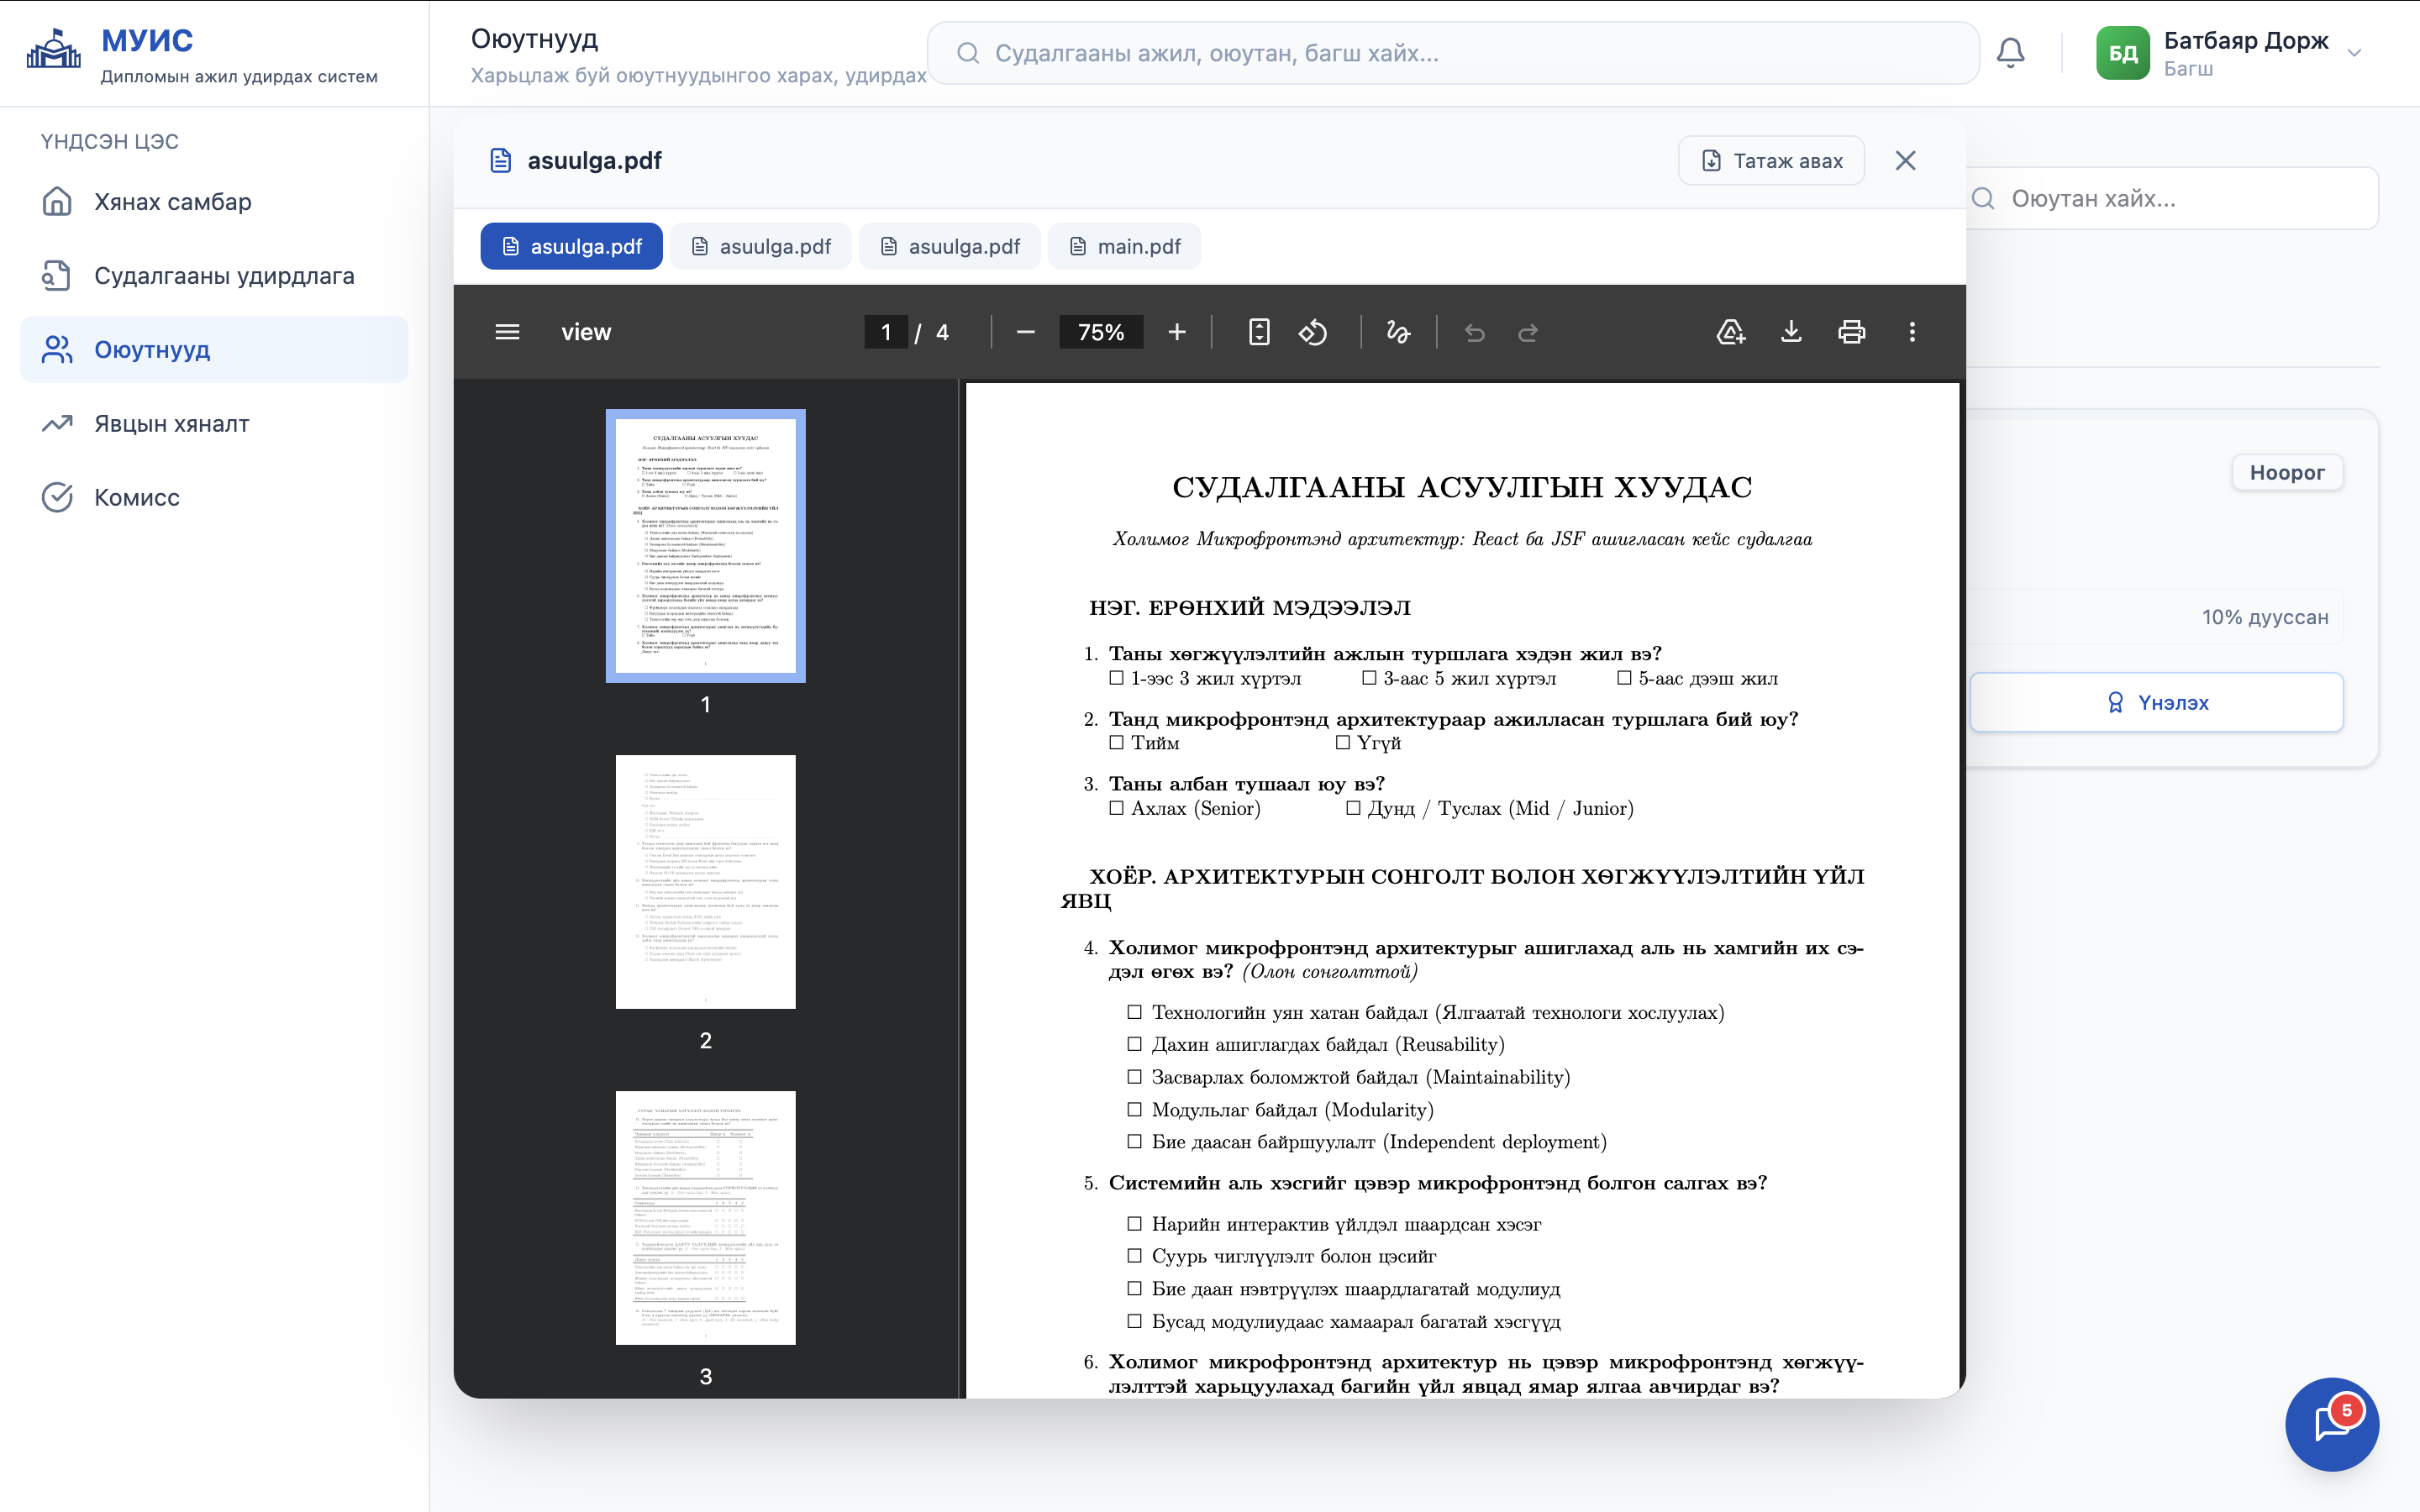
\includegraphics[width=16cm]{images/mf3.png}
  \caption{Оюутны илгээсэн тайланг хянах хэсэг}
  \label{fig:p3}
\end{figure}
\begin{figure}[H]
  \centering
  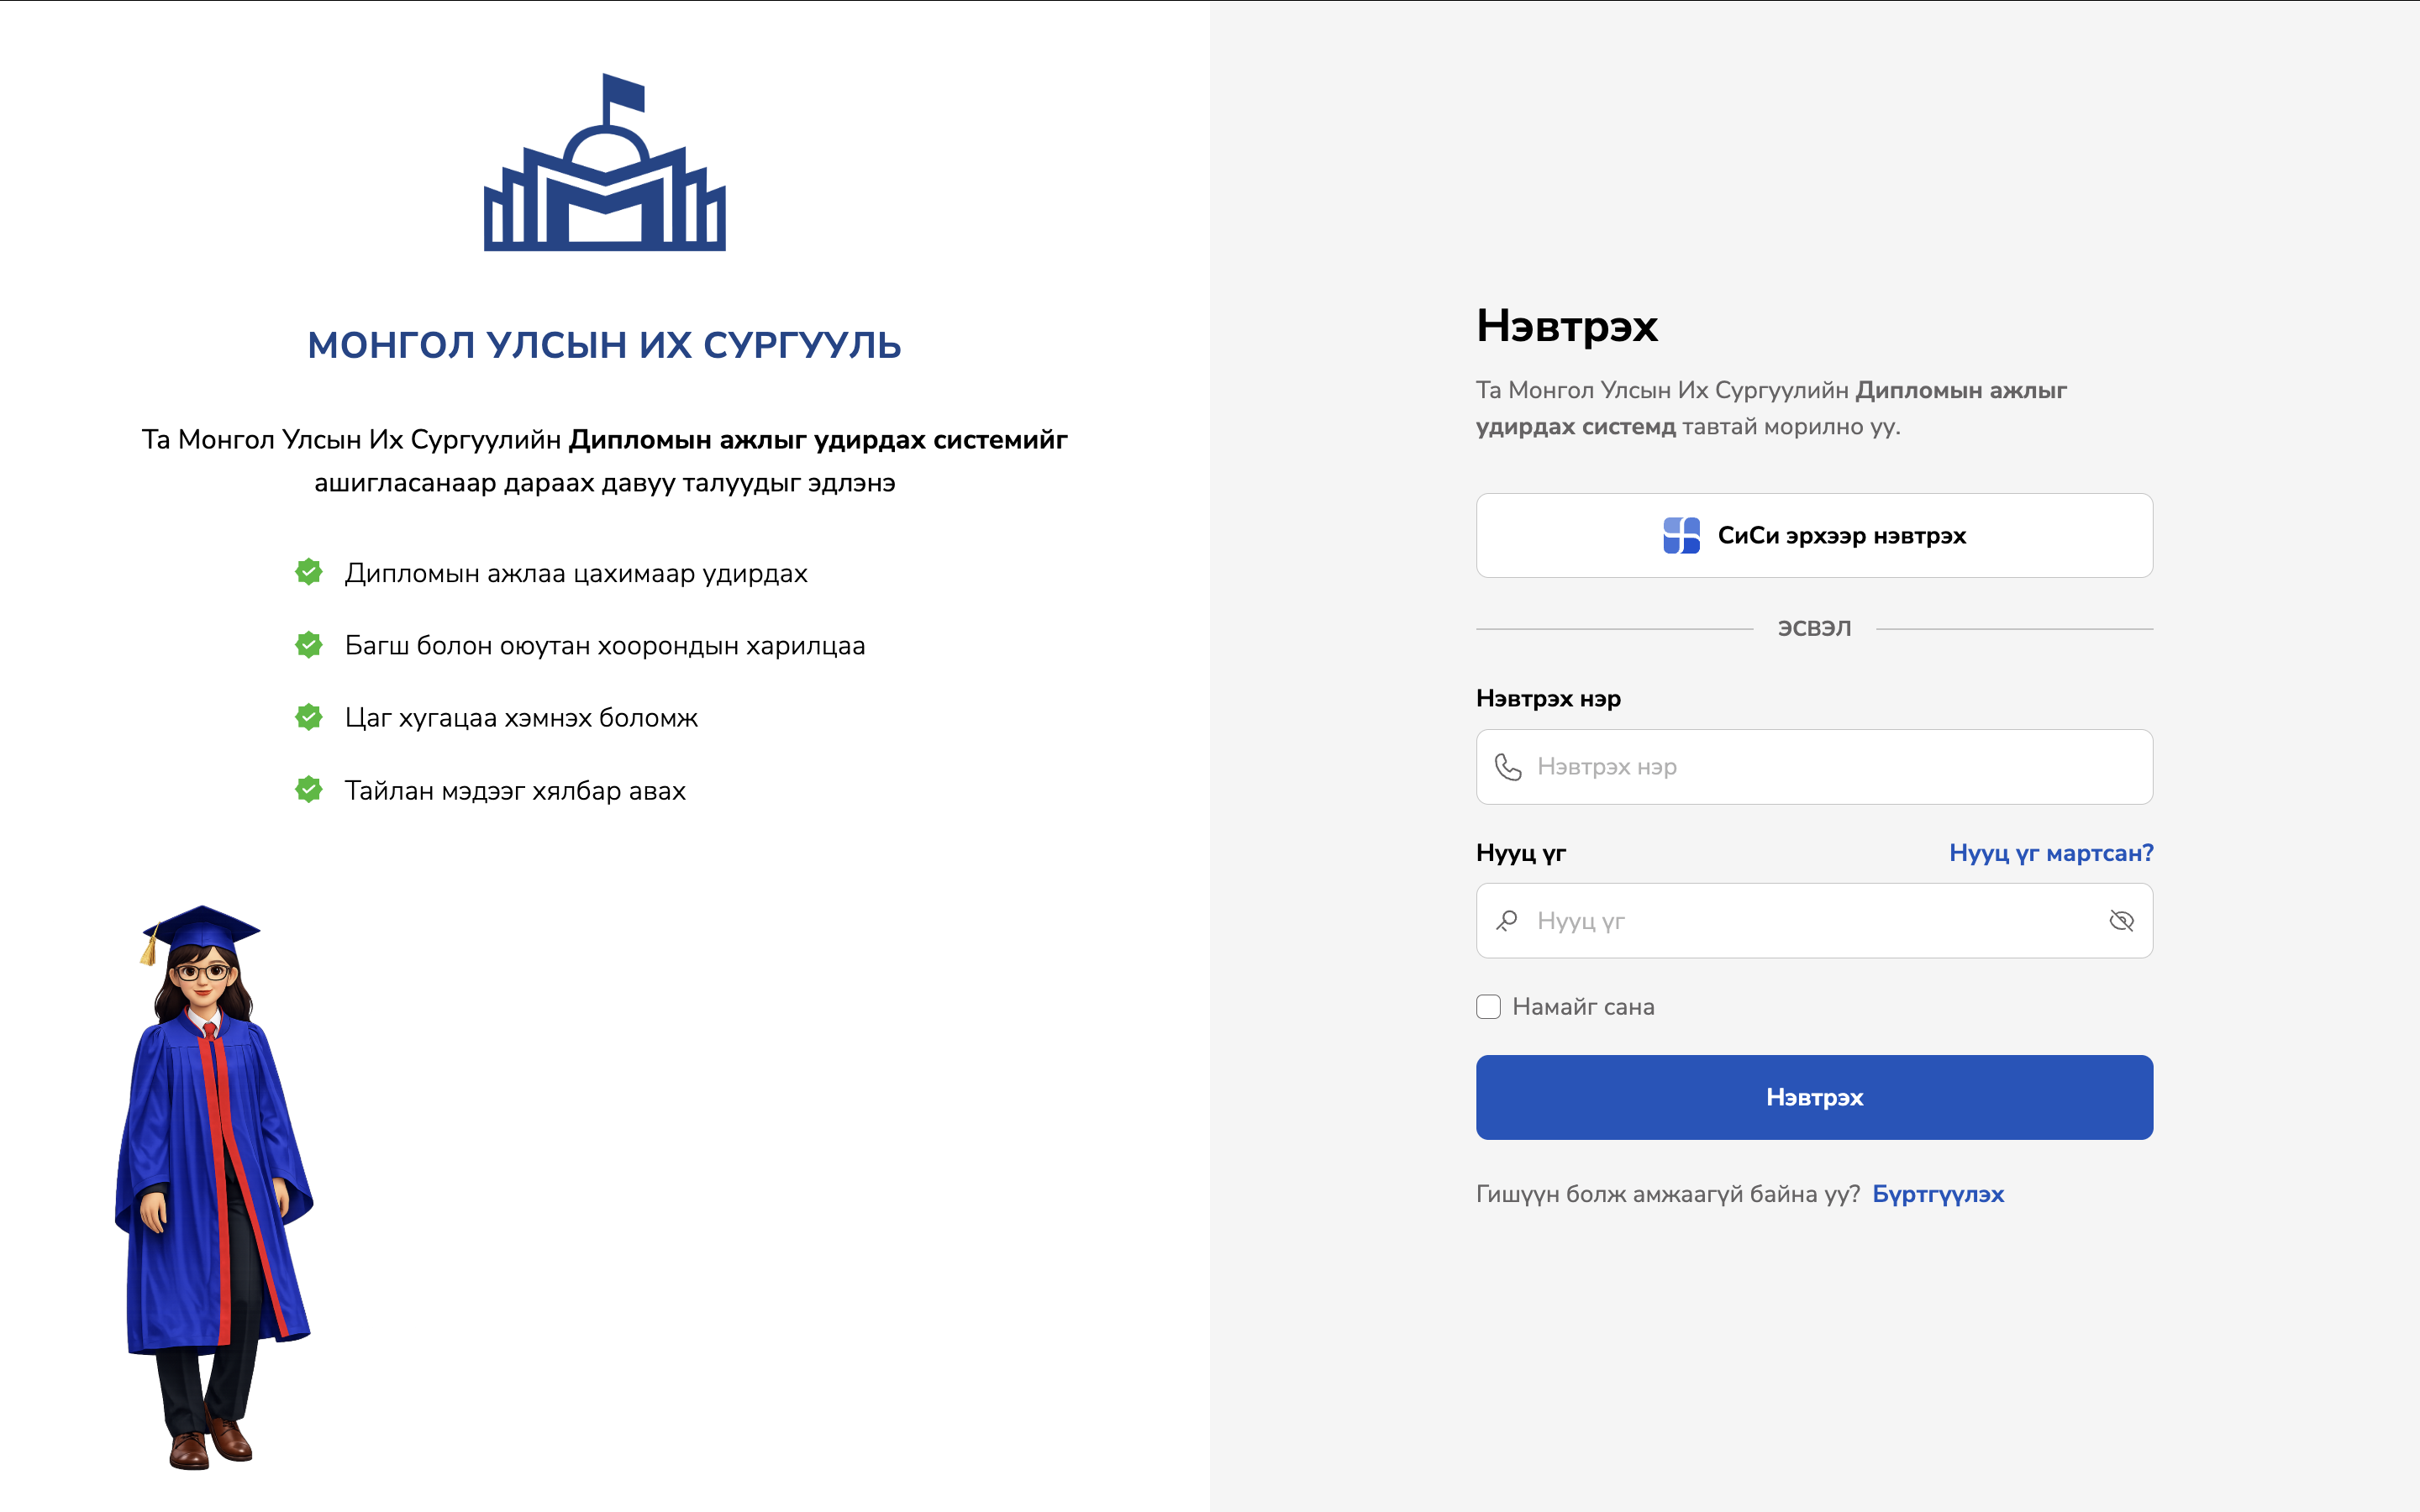
\includegraphics[width=16cm]{images/mf4.png}
  \caption{Системд нэвтрэх цонх}
  \label{fig:p4}
\end{figure}
\begin{figure}[H]
  \centering
  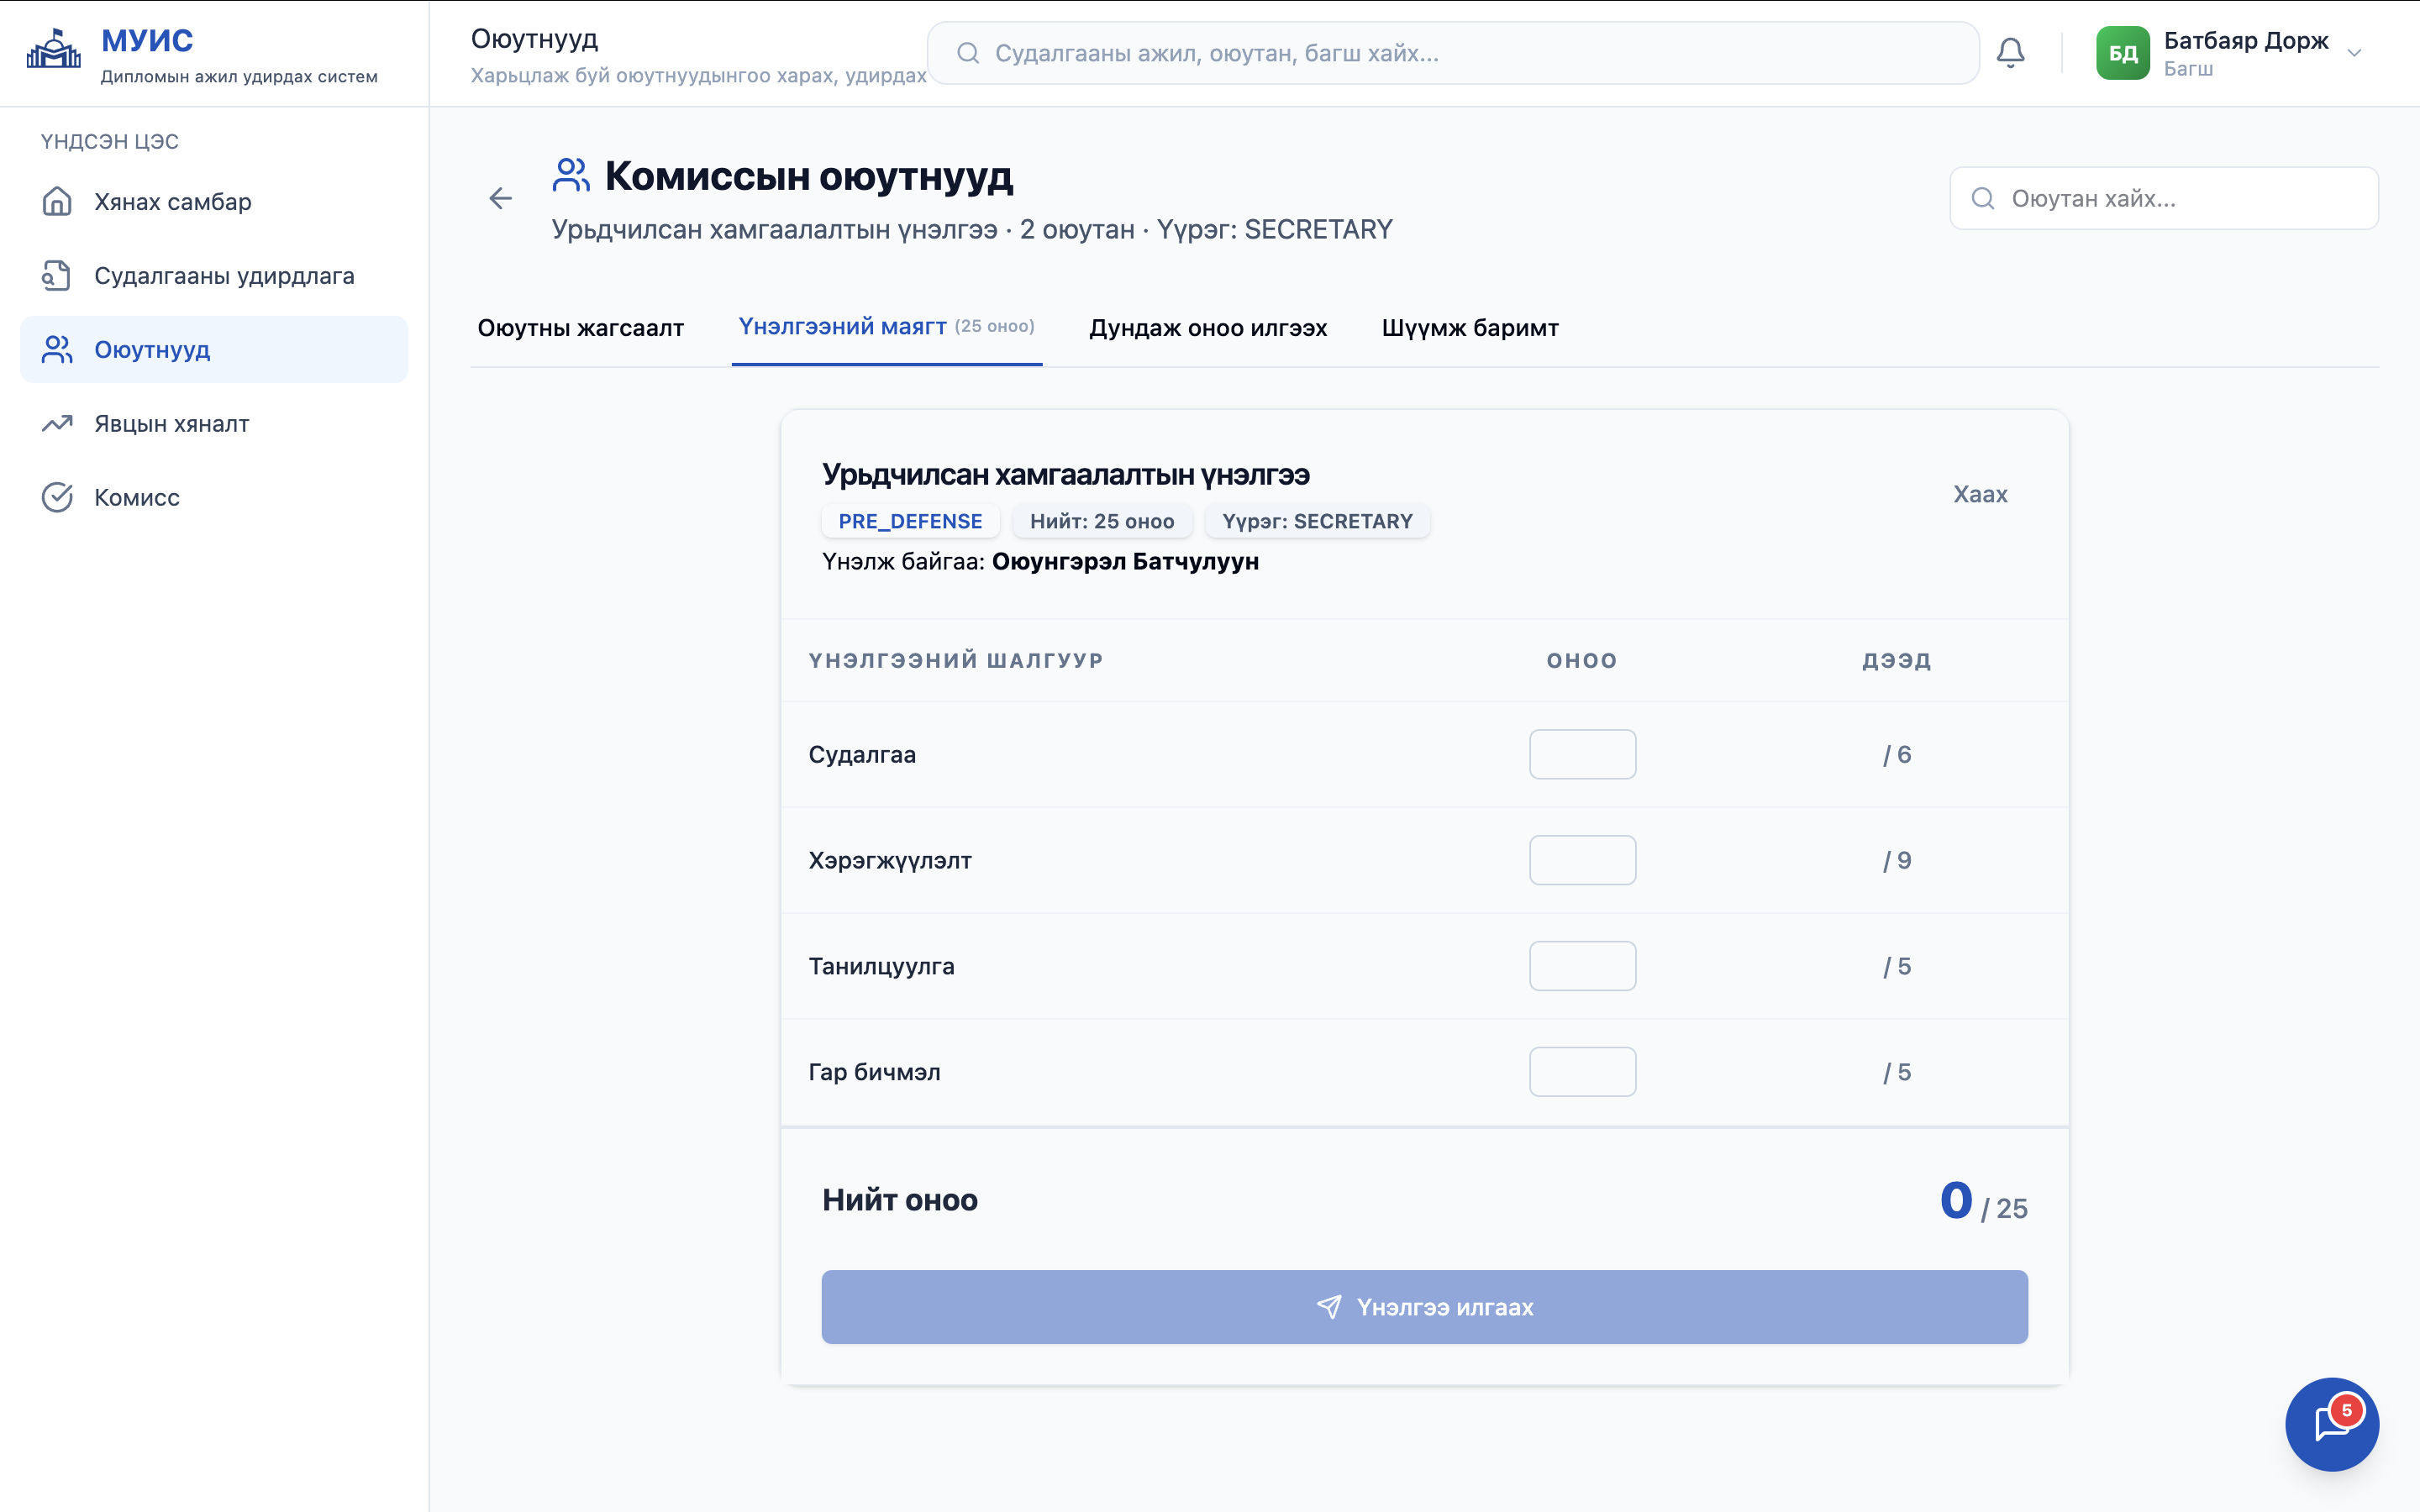
\includegraphics[width=16cm]{images/mf5.png}
  \caption{Комиссын гишүүн оюутны ажлыг үнэлэх хэсэг}
  \label{fig:p}
\end{figure}
\begin{figure}[H]
  \centering
  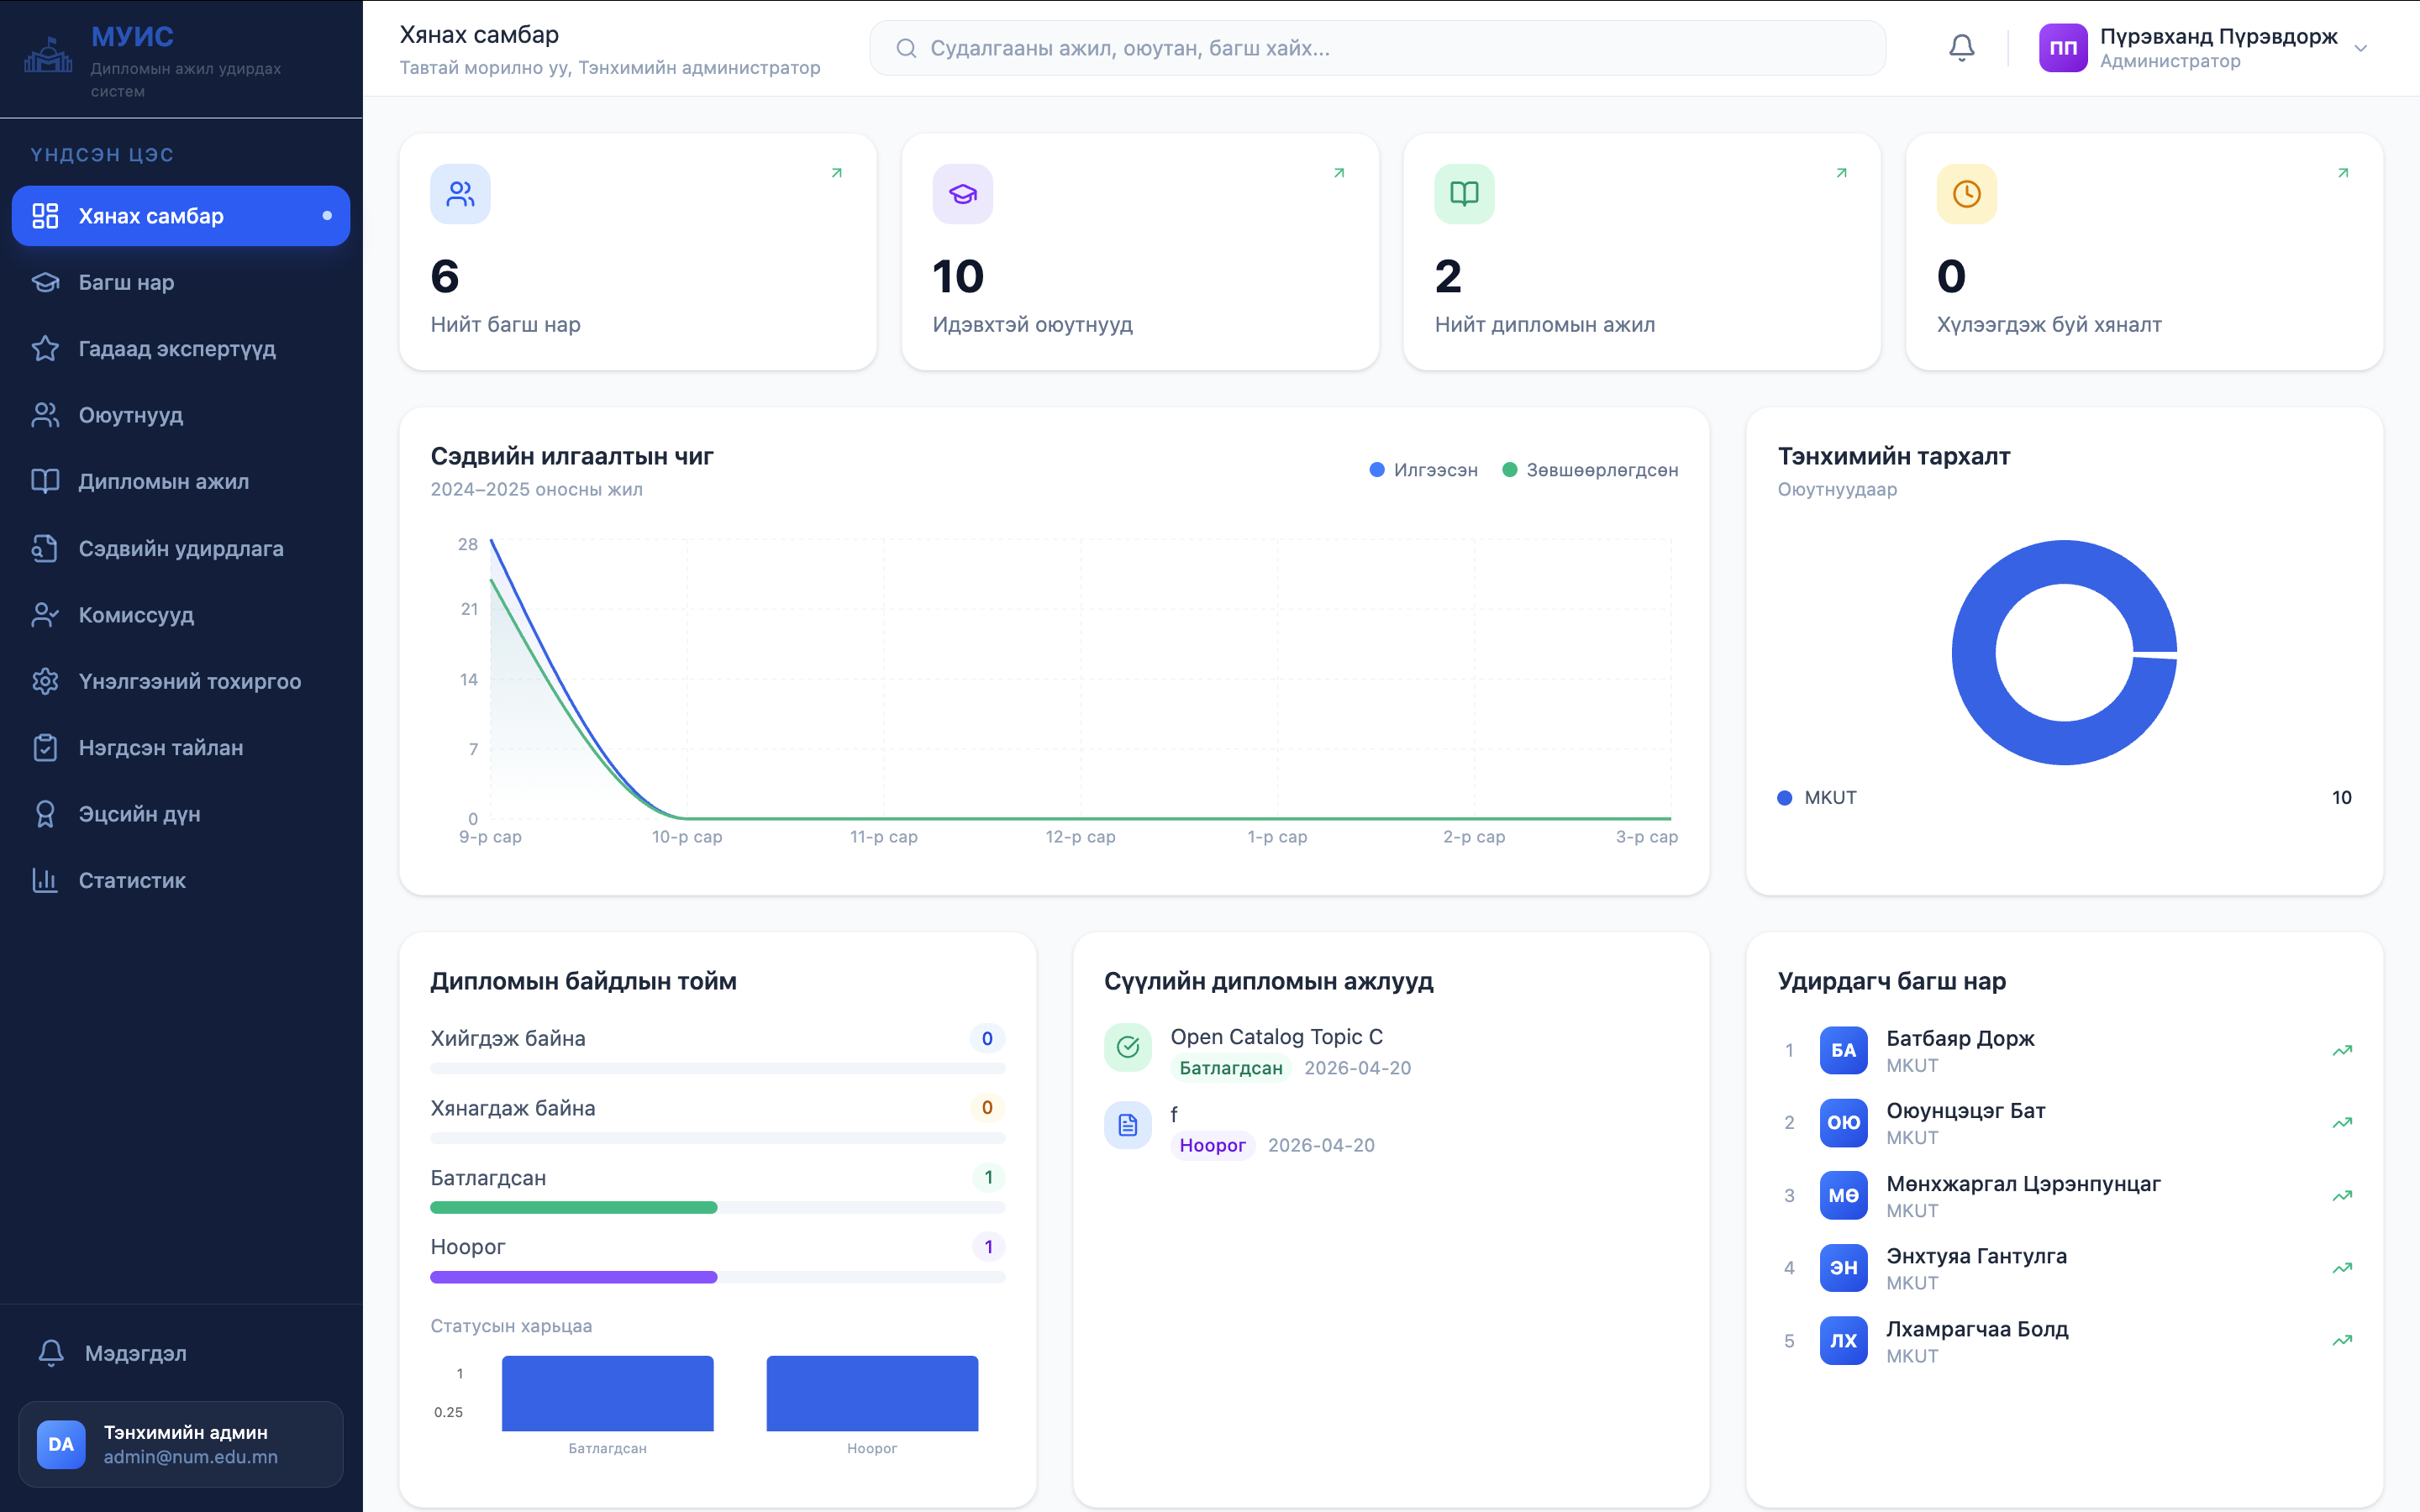
\includegraphics[width=16cm]{images/mf6.png}
  \caption{Тэнхимийн хянах самбар}
  \label{fig:p6}
\end{figure}
\begin{figure}[H]
  \centering
  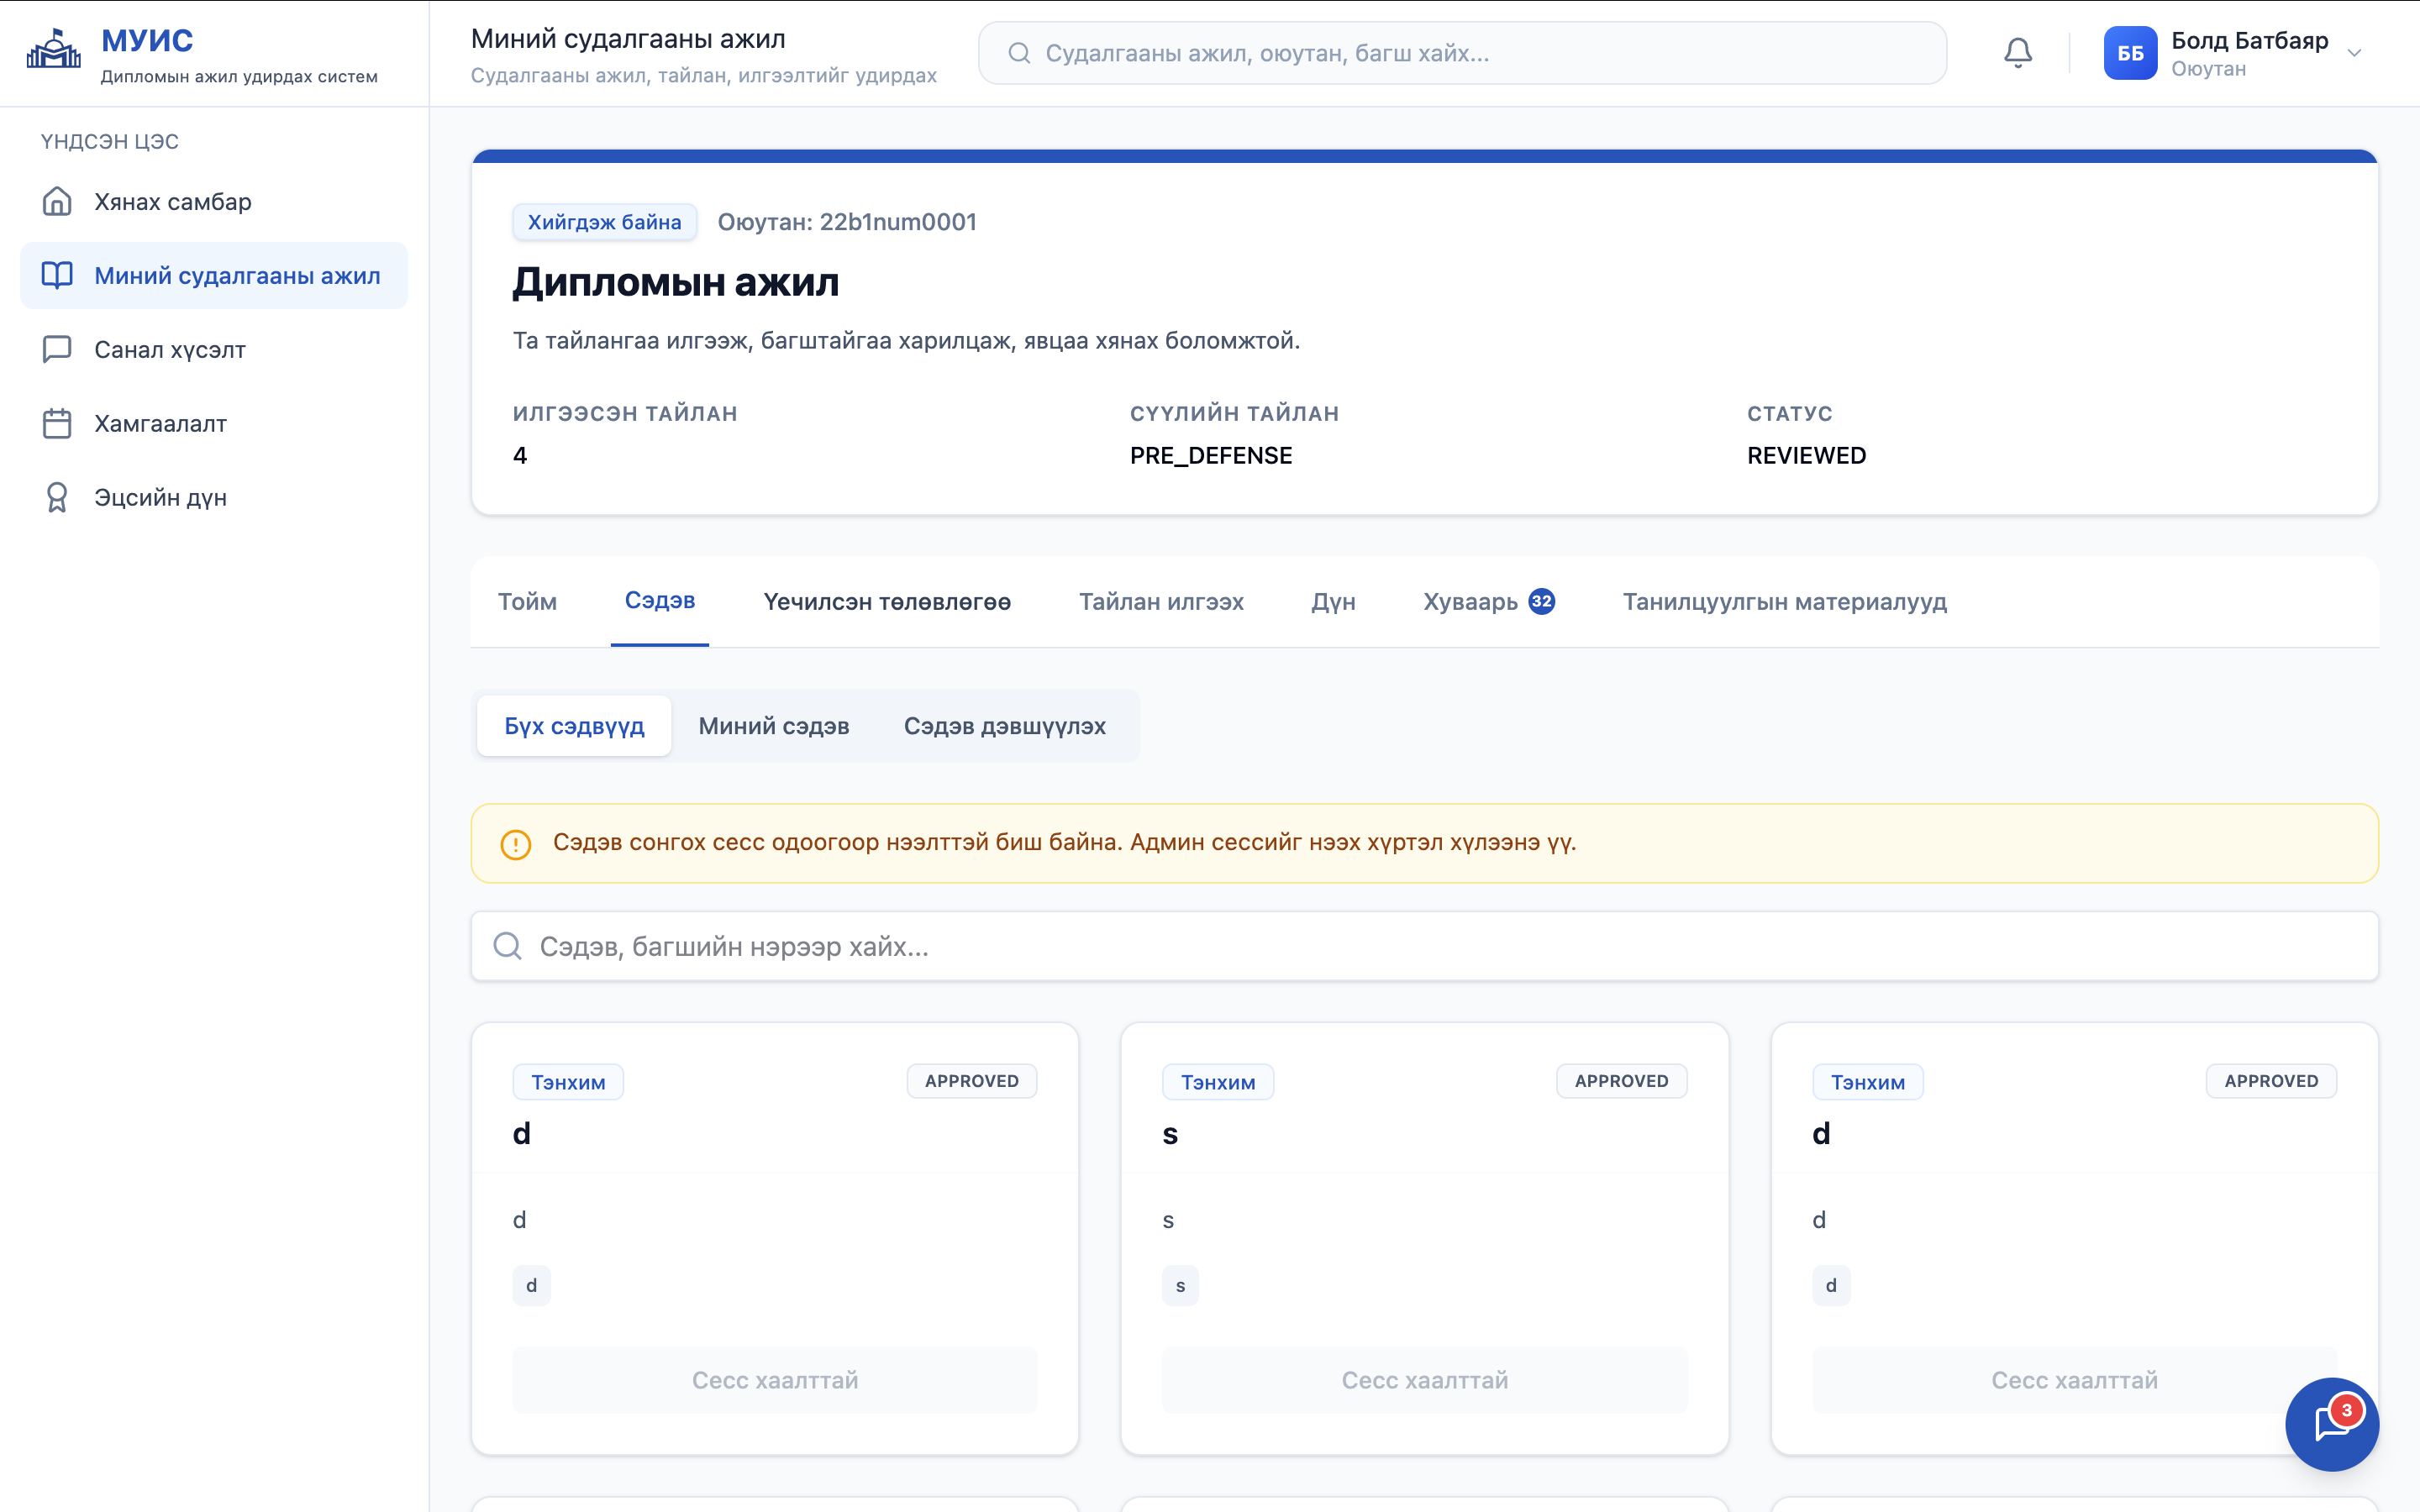
\includegraphics[width=16cm]{images/mf7.png}
  \caption{Сэдэ сонголтын хэсэг}
  \label{fig:p7}
\end{figure}
\begin{figure}[H]
  \centering
  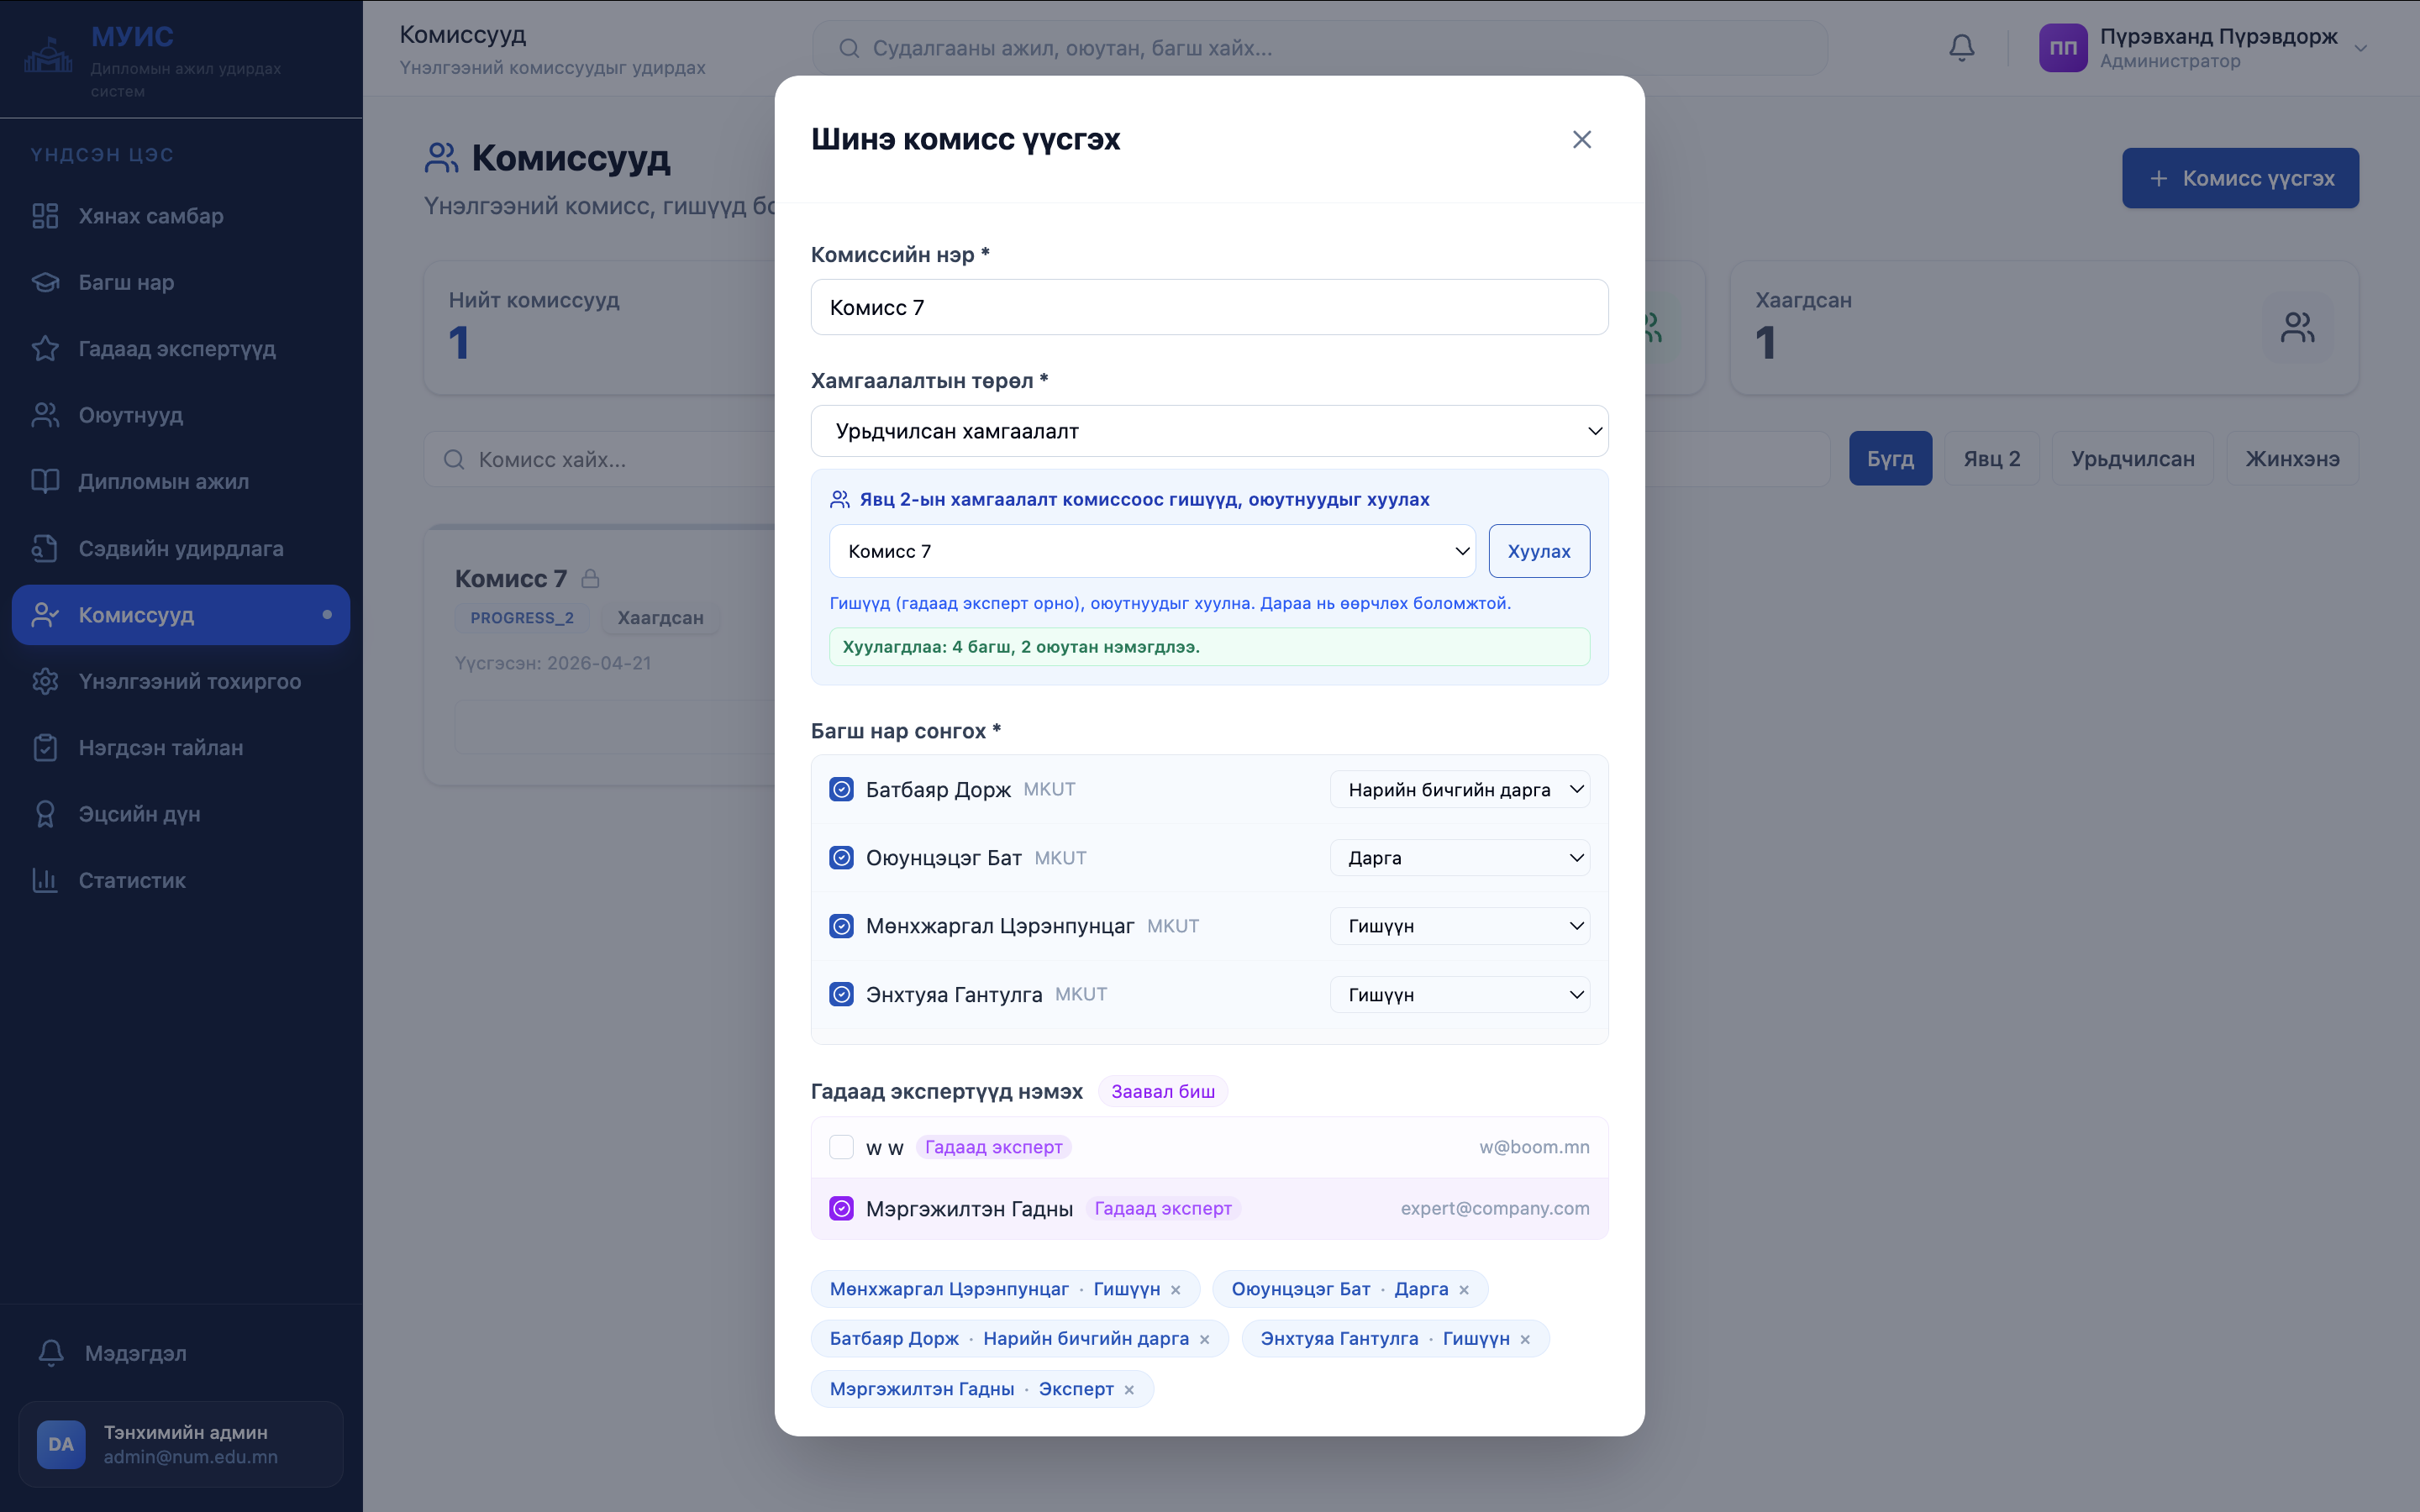
\includegraphics[width=16cm]{images/mf8.png}
  \caption{Комисс үүсгэх хэсэг}
  \label{fig:p8}
\end{figure}
\begin{figure}[H]
  \centering
  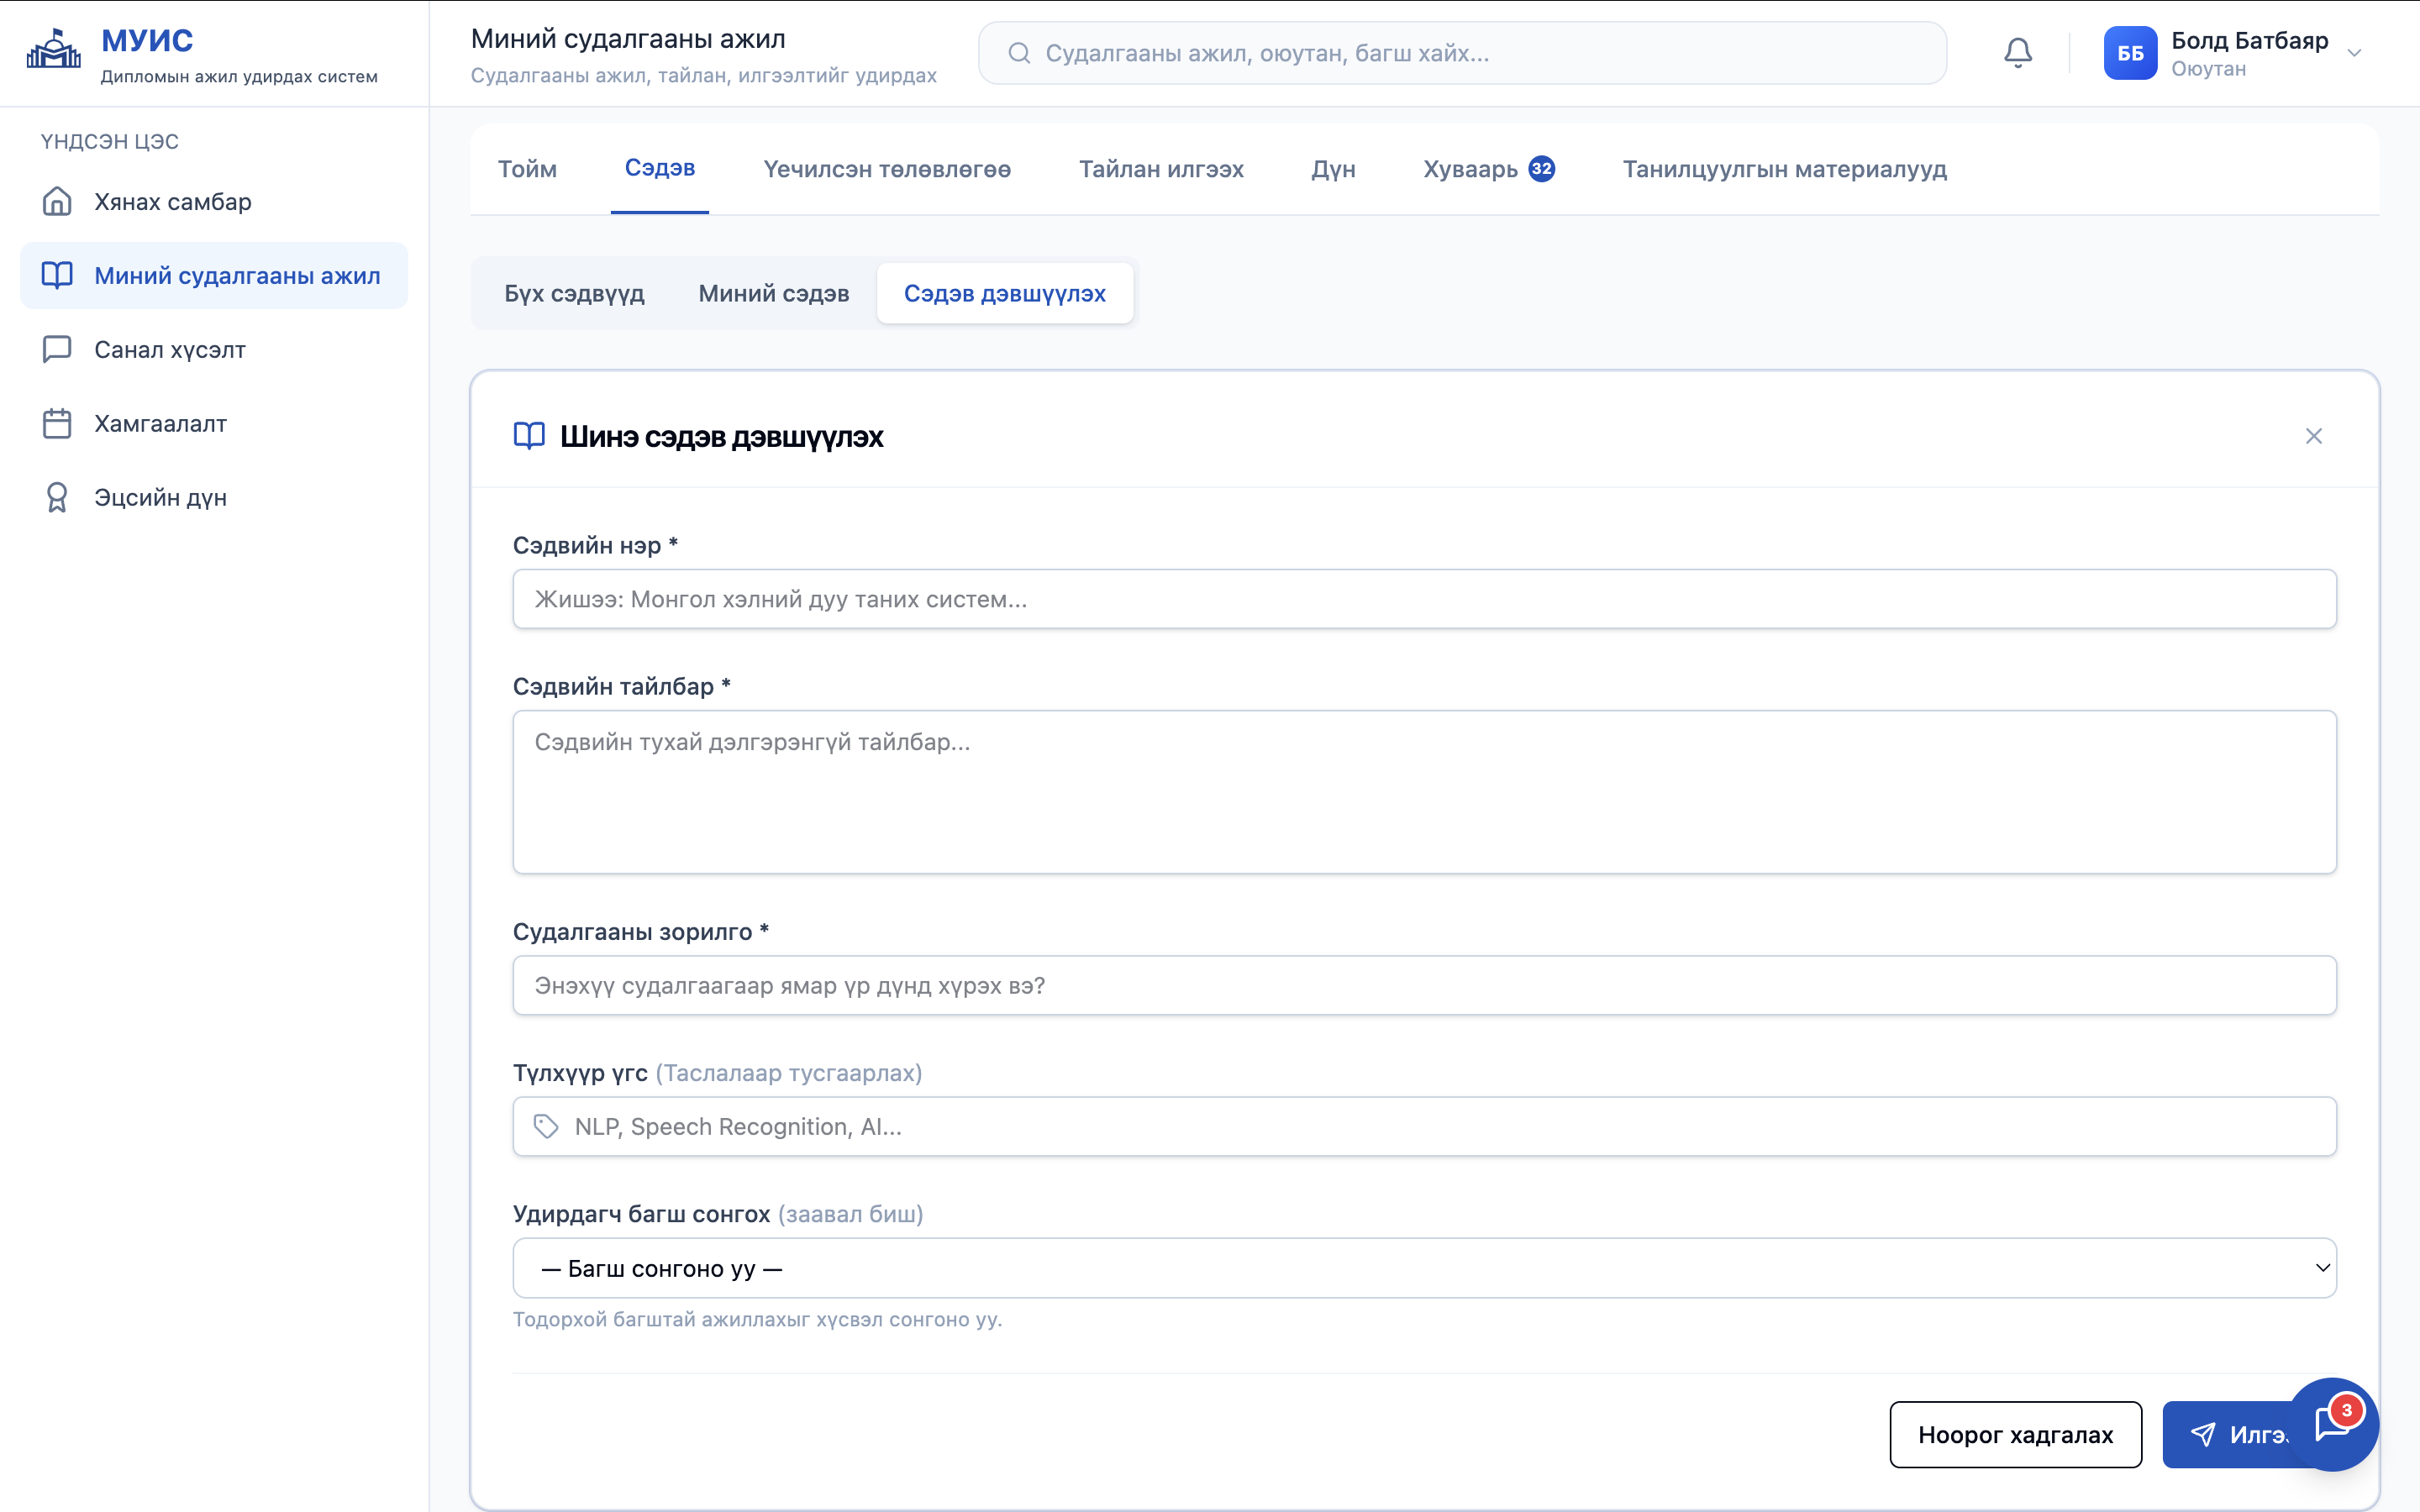
\includegraphics[width=16cm]{images/mf9.png}
  \caption{Оюутан сэдэв дэвшүүлэх хэсэг}
  \label{fig:p9}
\end{figure}

%\subfile{chapters/appendixtable.tex}
\chapter{Кодын хэрэгжүүлэлт}
\begin{lstlisting}[language=Java, caption={DefenseSessionController.java}, label={lst:c1}]
package mn.num.edu.workflow_service.adapters.in.web;

import mn.num.edu.workflow_service.adapters.out.persistence.entity.DefenseSessionEntity;
import mn.num.edu.workflow_service.adapters.out.persistence.repository.DefenseSessionR2dbcRepository;
import org.springframework.http.HttpStatus;
import org.springframework.http.ResponseEntity;
import org.springframework.web.bind.annotation.*;
import reactor.core.publisher.Flux;
import reactor.core.publisher.Mono;

import java.math.BigDecimal;
import java.time.LocalDateTime;
import java.util.Map;
import java.util.UUID;

@RestController
@RequestMapping("/api/defense-sessions")
public class DefenseSessionController {

    private final DefenseSessionR2dbcRepository repository;

    public DefenseSessionController(DefenseSessionR2dbcRepository repository) {
        this.repository = repository;
    }

    // Canonical DB stage names + frontend aliases
    private static final Map<String, BigDecimal> STAGE_MAX_POINTS = Map.of(
            "PROGRESS_1",    BigDecimal.valueOf(15),
            "PROGRESS_2",    BigDecimal.valueOf(20),
            "PRELIMINARY",   BigDecimal.valueOf(25),
            "PRE_DEFENSE",   BigDecimal.valueOf(25),
            "FINAL",         BigDecimal.valueOf(40),
            "FINAL_DEFENSE", BigDecimal.valueOf(40)
    );

    // Map frontend aliases to DB-accepted values
    private static String canonicalStageType(String stageType) {
        if ("PRE_DEFENSE".equals(stageType))   return "PRELIMINARY";
        if ("FINAL_DEFENSE".equals(stageType)) return "FINAL";
        return stageType;
    }

    @GetMapping
    public Flux<DefenseSessionEntity> listAll(@RequestParam(required = false) String committeeId,
                                              @RequestParam(required = false) String departmentId,
                                              @RequestParam(required = false) String status) {
        if (committeeId != null) return repository.findByCommitteeId(committeeId);
        if (departmentId != null) return repository.findByDepartmentId(departmentId);
        if (status != null) return repository.findByStatus(status);
        return repository.findAll();
    }

    @GetMapping("/{id}")
    public Mono<ResponseEntity<DefenseSessionEntity>> getById(@PathVariable String id) {
        return repository.findById(id)
                .map(ResponseEntity::ok)
                .defaultIfEmpty(ResponseEntity.notFound().build());
    }

    @GetMapping("/by-committee-stage")
    public Mono<ResponseEntity<DefenseSessionEntity>> getByCommitteeStage(
            @RequestParam String committeeId, @RequestParam String stageType) {
        return repository.findByCommitteeIdAndStageType(committeeId, stageType)
                .map(ResponseEntity::ok)
                .defaultIfEmpty(ResponseEntity.notFound().build());
    }

    @PostMapping
    public Mono<ResponseEntity<DefenseSessionEntity>> create(@RequestBody CreateDefenseSessionRequest req) {
        if (!STAGE_MAX_POINTS.containsKey(req.stageType())) {
            return Mono.just(ResponseEntity.badRequest().<DefenseSessionEntity>build());
        }
        String canonicalStage = canonicalStageType(req.stageType());
        BigDecimal maxPts = req.maxPoints() != null ? req.maxPoints() : STAGE_MAX_POINTS.get(req.stageType());

        DefenseSessionEntity entity = new DefenseSessionEntity();
        entity.setId(UUID.randomUUID().toString());
        entity.setNew(true);
        entity.setDepartmentId(req.departmentId() != null ? req.departmentId() : "GLOBAL");
        entity.setCommitteeId(req.committeeId() != null ? req.committeeId() : "GLOBAL");
        entity.setStageType(canonicalStage);
        entity.setMaxPoints(maxPts);
        entity.setStatus("PENDING");
        entity.setCreatedAt(LocalDateTime.now());

        return repository.save(entity)
                .map(saved -> ResponseEntity.status(HttpStatus.CREATED).body(saved))
                .onErrorResume(org.springframework.dao.DuplicateKeyException.class, e ->
                        repository.findByCommitteeIdAndStageType(entity.getCommitteeId(), canonicalStage)
                                .map(existing -> ResponseEntity.ok(existing))
                                .defaultIfEmpty(ResponseEntity.status(HttpStatus.CONFLICT).<DefenseSessionEntity>build())
                );
    }

    @PatchMapping("/{id}/open")
    public Mono<ResponseEntity<DefenseSessionEntity>> open(@PathVariable String id,
                                                           @RequestBody(required = false) OpenCloseRequest req) {
        String actor = req != null && req.actorId() != null ? req.actorId() : "admin";
        return repository.findById(id)
                .switchIfEmpty(Mono.error(new IllegalArgumentException("Defense session not found")))
                .flatMap(e -> {
                    e.setStatus("ACTIVE");
                    e.setStartedBy(actor);
                    e.setStartedAt(LocalDateTime.now());
                    e.setNew(false);
                    return repository.save(e);
                })
                .map(ResponseEntity::ok);
    }

    @PatchMapping("/{id}/close")
    public Mono<ResponseEntity<DefenseSessionEntity>> close(@PathVariable String id,
                                                            @RequestBody(required = false) OpenCloseRequest req) {
        String actor = req != null && req.actorId() != null ? req.actorId() : "admin";
        return repository.findById(id)
                .switchIfEmpty(Mono.error(new IllegalArgumentException("Defense session not found")))
                .flatMap(e -> {
                    e.setStatus("CLOSED");
                    e.setClosedBy(actor);
                    e.setClosedAt(LocalDateTime.now());
                    e.setNew(false);
                    return repository.save(e);
                })
                .map(ResponseEntity::ok);
    }

    public record CreateDefenseSessionRequest(String departmentId, String committeeId,
                                               String stageType, BigDecimal maxPoints) {}
    public record OpenCloseRequest(String actorId) {}
}
\end{lstlisting}

\begin{lstlisting}[language=Java, caption={CorsConfig.java}, label={lst:c2}]
package mn.num.edu.workflow_service.config;

import org.springframework.context.annotation.Bean;
import org.springframework.context.annotation.Configuration;
import org.springframework.web.cors.CorsConfiguration;
import org.springframework.web.cors.reactive.CorsWebFilter;
import org.springframework.web.cors.reactive.UrlBasedCorsConfigurationSource;

import java.util.List;

@Configuration
public class CorsConfig {

    @Bean
    public CorsWebFilter corsWebFilter() {
        CorsConfiguration config = new CorsConfiguration();
        config.setAllowedOriginPatterns(List.of("*"));
        config.setAllowedMethods(List.of("GET", "POST", "PUT", "PATCH", "DELETE", "OPTIONS"));
        config.setAllowedHeaders(List.of("*"));
        config.setAllowCredentials(true);
        UrlBasedCorsConfigurationSource source = new UrlBasedCorsConfigurationSource();
        source.registerCorsConfiguration("/**", config);
        return new CorsWebFilter(source);
    }
}
\end{lstlisting}

\begin{lstlisting}[language=JavaScript, caption={vite.config.ts}, label={lst:c3}]
import { defineConfig } from 'vite';
import path from 'path';
import react from '@vitejs/plugin-react';
import tailwindcss from '@tailwindcss/vite';
import federation from '@originjs/vite-plugin-federation';
const TOMCAT = 'http://localhost:8080/microfrontends';
export default defineConfig(({ command }) => {
  const isProd = command === 'build';
  const sharedUiUrl = isProd
    ? `${TOMCAT}/shared-ui-module/dist/remoteEntry.js`
    : 'http://localhost:3020/remoteEntry.js';
  const moduleThesisUrl = isProd
    ? `${TOMCAT}/module-thesis/dist/remoteEntry.js`
    : 'http://localhost:3013/remoteEntry.js';
  return {
    base: '/microfrontends/module-teacher/dist/',
    plugins: [
      react(),
      tailwindcss(),
      federation({
        name: 'module_teacher',
        remotes: {
          shared_ui:     sharedUiUrl,
          module_thesis: moduleThesisUrl,
        },
        shared: {
          react:       { singleton: true, requiredVersion: '18.3.1' },
          'react-dom': { singleton: true, requiredVersion: '18.3.1' },
          antd:        { singleton: true, requiredVersion: '^5.22.0' },
        },
      }),
    ],
    resolve: {
      alias: { '@': path.resolve(__dirname, './src') },
    },
    css: {
      modules: {
        generateScopedName: 'mtch_[local]_[hash:6]',
      },
    },
    build: {
      target: 'esnext',
      minify: false,
      cssCodeSplit: false,
      outDir: 'dist',
      rollupOptions: {
        input: path.resolve(__dirname, 'src/index.ts'),
        output: {
          entryFileNames: 'main.js',
          chunkFileNames: 'chunk-[name].js',
          assetFileNames: '[name][extname]',
          minifyInternalExports: false,
        },
      },
    },
  };
});
\end{lstlisting}

\begin{lstlisting}[language=JavaScript, caption={AuthContext.tsx}, label={lst:c4}]
import { createContext, useContext, useState, useEffect, ReactNode } from 'react';
import { mockLoginWithStored, mockRegister, UserRole, ROLE_REDIRECT_MAP } from '@/services/mockAuthService';

const AUTH_API  = 'http://localhost:8887';
const USER_API  = 'http://localhost:8086';

interface AuthUser {
  username: string;
  displayName: string;
  role: UserRole;
}

interface AuthContextType {
  user: AuthUser | null;
  isAuthenticated: boolean;
  login: (username: string, password: string, rememberMe: boolean) => Promise<{ success: boolean; error?: string }>;
  register: (username: string, password: string, role?: UserRole) => Promise<{ success: boolean; error?: string }>;
  logout: () => void;
}

const AuthContext = createContext<AuthContextType | undefined>(undefined);

const STORAGE_KEY = 'mauth_current_user';

function mapRole(roles: string[]): UserRole {
  if (!roles || roles.length === 0) return 'student';
  const r = roles[0].toUpperCase();
  if (r.includes('ADMIN'))   return 'admin';
  if (r.includes('TEACHER')) return 'teacher';
  return 'student';
}
async function realLogin(sisiId: string, password: string): Promise<{ success: boolean; user?: AuthUser; error?: string }> {
  try {
    const res = await fetch(`${AUTH_API}/auth/login`, {
      method: 'POST',
      headers: { 'Content-Type': 'application/json' },
      body: JSON.stringify({ sisiId: sisiId.trim(), password }),
    });
    if (!res.ok) {
      return { success: false, error: 'Нэвтрэх нэр эсвэл нууц үг буруу байна' };
    }
    const data = await res.json();
    const role = mapRole(data.roles ?? []);
    localStorage.setItem('mauth_token', data.token ?? '');
    const resolvedSisiId = data.sisiId ?? sisiId;
    let displayName = resolvedSisiId;
    try {
      const emailCandidates = [
        `${resolvedSisiId}@stud.num.edu.mn`,
        `${resolvedSisiId}@num.edu.mn`,
      ];
      for (const email of emailCandidates) {
        const userRes = await fetch(`${USER_API}/api/users/by-email?email=${encodeURIComponent(email)}`);
        if (userRes.ok) {
          const userProfile = await userRes.json();
          const first = userProfile.firstName ?? '';
          const last  = userProfile.lastName  ?? '';
          if (first || last) { displayName = `${first} ${last}`.trim(); }
          break;
        }
      }
    } catch {
      // user_service unavailable — keep sisiId as name
    }
    return {
      success: true,
      user: { username: resolvedSisiId, displayName, role },
    };
  } catch {
    return { success: false, error: '__NETWORK_ERROR__' };
  }
}
export function AuthProvider({ children }: { children: ReactNode }) {
  const [user, setUser] = useState<AuthUser | null>(null);
  useEffect(() => {сэргээнэ
    const saved =
      localStorage.getItem(STORAGE_KEY) || sessionStorage.getItem(STORAGE_KEY);
    if (saved) {
      try {
        setUser(JSON.parse(saved));
      } catch {
        localStorage.removeItem(STORAGE_KEY);
        sessionStorage.removeItem(STORAGE_KEY);
      }
    }
  }, []);
  const login = async (username: string, password: string, rememberMe: boolean) => {
    const realResult = await realLogin(username, password);
    let userData: AuthUser | null = null;
    if (realResult.success && realResult.user) {
      userData = realResult.user;
    } else if (realResult.error === '__NETWORK_ERROR__') {
      const mockResult = await mockLoginWithStored(username, password);
      if (mockResult.success && mockResult.user) {
        userData = {
          username: mockResult.user.username,
          displayName: mockResult.user.displayName,
          role: mockResult.user.role,
        };
      } else {
        return { success: false, error: mockResult.error };
      }
    } else {
      return { success: false, error: realResult.error };
    }
    setUser(userData);
    const storage = rememberMe ? localStorage : sessionStorage;
    storage.setItem(STORAGE_KEY, JSON.stringify(userData));
    const redirectUrl = ROLE_REDIRECT_MAP[userData.role];
    window.location.href = redirectUrl;
    return { success: true };
  };
  const register = async (username: string, password: string, role: UserRole = 'student') => {
    const result = await mockRegister(username, password, role);
    if (result.success) {
      return { success: true };
    }
    return { success: false, error: result.error };
  };
  const logout = () => {
    setUser(null);
    localStorage.removeItem(STORAGE_KEY);
    sessionStorage.removeItem(STORAGE_KEY);
    window.location.href = '/login.xhtml';
  };
  return (
    <AuthContext.Provider value={{ user, isAuthenticated: !!user, login, register, logout }}>
      {children}
    </AuthContext.Provider>
  );
}
export function useAuth() {
  const ctx = useContext(AuthContext);
  if (!ctx) throw new Error('useAuth must be used within AuthProvider');
  return ctx;
}
\end{lstlisting}

\begin{lstlisting}[language=JavaScript, caption={authGuard.ts}, label={lst:c5}]
/**
 * authGuard.ts — Микрофронтэндийн нэвтрэлт болон дүрийн хамгаалалт
 *
 * Архитектурын тэмдэглэл:
 * - Нэвтрэлтийн мэдээлэл localStorage-д хадгалагддаг (module-auth тохируулна)
 * - Дүр тус бүрийн модуль mount хийхдээ энэ функцийг дуудна
 * - Нэвтрэлт байхгүй → login.xhtml руу redirect
 * - Буруу дүр → өөрийн дүрийн хуудас руу redirect
 */

export type UserRole = 'admin' | 'teacher' | 'student';

export interface StoredUser {
  username: string;
  displayName: string;
  role: UserRole;
  userId?: string;
}

const STORAGE_KEY = 'mauth_current_user';

/** localStorage-аас нэвтэрсэн хэрэглэгчийг унших */
export function getStoredUser(): StoredUser | null {
  try {
    const raw =
      localStorage.getItem(STORAGE_KEY) ||
      sessionStorage.getItem(STORAGE_KEY);
    if (!raw) return null;
    return JSON.parse(raw) as StoredUser;
  } catch {
    return null;
  }
}

/** Нэвтрэлт болон дүрийг шалгаж, шаардлагатай бол redirect хийнэ */
export function guardRoute(requiredRole: UserRole): StoredUser | null {
  const user = getStoredUser();

  // Нэвтрээгүй бол login хуудас руу
  if (!user) {
    window.location.replace('/login.xhtml');
    return null;
  }

  // Дүр буруу бол өөрийн хуудас руу
  if (user.role !== requiredRole) {
    const redirectMap: Record<UserRole, string> = {
      admin: '/admin.xhtml',
      teacher: '/teacher.xhtml',
      student: '/student.xhtml',
    };
    window.location.replace(redirectMap[user.role]);
    return null;
  }

  return user;
}

/** Гарах — localStorage цэвэрлэж login руу шилжих */
export function logout(): void {
  localStorage.removeItem(STORAGE_KEY);
  sessionStorage.removeItem(STORAGE_KEY);
  window.location.replace('/login.xhtml');
}
\end{lstlisting}